\chapter{Métricas}

Dentre as várias formas que um gerente de projeto tem a sua disposição para acompanhar o andamento de um 
projeto destaca-se o uso do gráfico \textit{Big Chart}. O mesmo pode ser visto como a análise quantitativa do 
andamento do projeto. As métricas a serem apresentadas são escolhidas pelo gerente e buscam refletir que 
pontos deseja-se acompanhar, por exemplo, se número de classes, número de linhas de código, testes de unidade 
que estão rodando perfeitamente, etc. As métricas escolhidas pela equipe em questão foram:

\begin{itemize}
 \item Número de Módulos python
 \item Número de scripts
 \item Número de Scritps de Testes de Aceitação Implementados e Executando Corretamente
 \item Número de Módulos de Testes de Unidade Implementados e Executando Corretamente
 \item Número de User Stories Finalizadas
 \item Total de Linhas de Código
 \item Total de Linhas de Teste
\end{itemize}


Vale ressaltar que o \textit{Big Chart} faz parte da documentação especificada em alguns processos vistos
 na academia como o \textit{YP} \cite{yp} e o \textit{XP1} \cite{xp1}. Como o processo de desenvolvimento 
escolhido durante as disciplinas de Projeto I e Projeto II foi baseado no \textit{XP1}, o \textit{Big Chart} 
foi utilizado para acompanhamento em alto nível do projeto por parte do cliente, bem como dos integrantes da 
equipe de desenvolvimento.

Uma vez que as iterações foram definidas com duração de 15 dias e uma \textit{release} contemplou, em média, duas 
iterações, optou-se em Projeto I por gerar as métricas a cada \textit{release}. Entretanto, como no final da disciplina 
surgiu um grave problema de convergência no resultado das fórmulas que estavam sendo usadas até então, 
optou-se por alterar o intervalo de atualização do mesmo, passando agora a atualizá-lo a cada 15 dias. Com 
isso buscou-se um maior controle sobre o status do projeto.

\begin{figure}[!h]
\centering
\subfigure[Métricas Gerais\label{fig:geral}]
{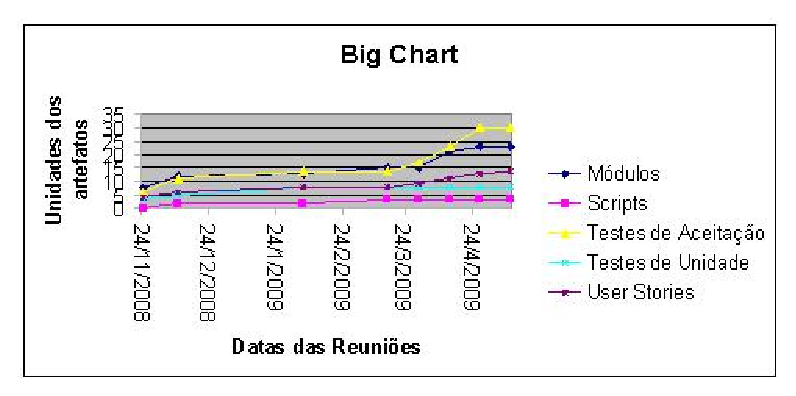
\includegraphics[scale = .8]{bc.eps}}
\subfigure[Linhas de código\label{fig:loc}]
{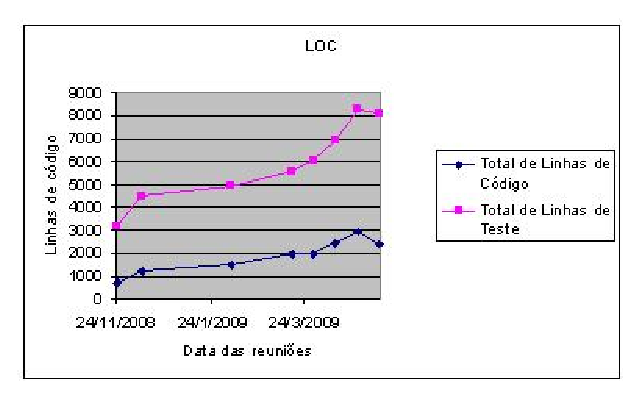
\includegraphics[scale = .8]{bc2.eps}}
%  \includegraphics[scale=0.5]{bigchart.eps}
 \caption{\it Big Chart.} \label{fig:bigchart}
\end{figure}

Conforme pode-se observar nas Figuras \ref{fig:geral} e \ref{fig:loc}, o desenvolvimento apresentou-se crescente
 até os meses de Fevereiro e Março quando o problema acima citado foi encontrado. Nesse instante foi 
realizado uma pesquisa por novas fórmulas, com teste das mesmas, o que levou a uma estabilidade tanto no 
total de linhas de código, como no número de módulos, testes de aceitação, testes de unidade e 
\textit{user stories}. Nesse mesmo intervalo o aumento no total de linhas de teste se deve à especificação
 de uma maior quantidade de testes de modo a garantir uma maior convergência com os resultados da HP-12C.

Durante o mês de Março, uma vez encontrado um conjunto de fórmulas que propiciou uma convergência adequada, 
iniciou-se o desenvolvimento das demais \textit{user stories} em questão e por isso explica-se o crescimento
 das métricas avaliadas. O grande aumento do número de \textit{user stories} se deve ao fato que após a
resolução dos problemas com as fórmulas, um conjunto de pequenas \textit{user stories} foram contempladas pelo
desenvolvimento. Essas \textit{user stories} tratavam basicamente de funções fáceis de implementar, cujas
fórmulas já haviam sido encontradas. Optou-se por deixar a implementação dessas funções por último, porque \textit{XP1}
aconselha começar o desenvolvimento pelas funcionalidades mais importantes (nesse caso, mais difíceis de serem 
implementadas). Pode-se observar que o número de testes de aceitação também aumentou para apoiar as 
novas \textit{user stories}.

As últimas avaliações realizadas em Maio apresentam valores constantes na Figura 
\ref{fig:geral} dado que esse foi um período de refatoramento de código e testes, bem como de melhorias em 
aspectos da interface. É interessante ressaltar que as alterações aqui produzidas levaram a uma certa queda 
no total de linhas de código e testes, Figura \ref{fig:loc}, dado que foi observado certa redundância em trechos 
de código e teste, bem como o fato de que foram realizadas simplificações na interface, o que leva a um menor 
número de linhas de código.

Vale observar que o número de scripts não variou muito durante todo o projeto, pois
eles foram utilizados basicamente para \textit{deploy} da aplicação. Os scripts de teste estão contabilizados
nas métricas de testes de aceitação e de testes de unidade.

Outro ponto que merece explicação é o porquê da quantidade de linhas de teste ser tão superior à quantidade 
de linhas de código. Mediante o uso do framework QT e da linguagem Python, bem como da busca de uso de boas 
técnicas de programação e design, o código da aplicação tornou-se bastante enxuto e reduzido. Quanto aos 
testes, uma vez que buscou-se uma grande similaridade com os resultados da HP-12C, foi elaborada uma alta 
carga de testes, buscando contemplar a maior variedade de cenários possível no tempo de desenvolvimento proposto.